\documentclass[a4paper]{article}
\usepackage[utf8]{inputenc}
\usepackage[russian,english]{babel}
\usepackage[T2A]{fontenc}
\usepackage[left=10mm, top=20mm, right=18mm, bottom=15mm, footskip=10mm]{geometry}
\usepackage{indentfirst}
\usepackage{amsmath,amssymb}
\usepackage[italicdiff]{physics}
\usepackage{graphicx}
\usepackage{multirow}
\usepackage{svg}
\graphicspath{{images/}}
\DeclareGraphicsExtensions{.pdf,.png,.jpg}
\usepackage{wrapfig}
\usepackage{caption}
\captionsetup[figure]{name=Рисунок}
\captionsetup[table]{name=Таблица}
\title{\underline{Скин эффект}}
\author{Каспаров Николай, Б01-304}

\begin{document}

\maketitle
\begin{center}
\Large{\textbf{ }}
\end{center}

\subparagraph{Цель работы:}

    исследовать явление проникновение переменного магнитного поля в медный полый цилиндр

\subparagraph{В работе используются:}

Генератор сигналов; соленоид, намотанный на полый цилиндрический каркас;
медный экран в виде полого цилиндра; измерительная катушка; амперметр; вольтметр;
двухканальный осциллограф; RLC-метр.

\section{Ход работы}

Параметры установки:

\begin{equation*}
    a + h = (45.0 \pm 0.1) ~ \text{мм}
\end{equation*}
\begin{equation*}
    h = (1.5 \pm 0.1) ~ \text{мм}
\end{equation*}
\begin{equation*}
    \sigma \approx (5 \cdot 10^7) \frac{\text{см}}{\text{м}}
\end{equation*}
\begin{equation*}
    \nu = (2250 \pm 5) ~ \text{Гц}
\end{equation*}

\subsection{Измерения амплитуд в области низких частот}

В области низких частот толщина скин-слоя превосходит толщину образца $\delta \gg h$:

\begin{equation}
    \left(\frac{|H_1|}{|H_0|}\right)^2 = (\xi_0\xi)^2 \approx \frac{1}{1+\left(\frac{ah}{\delta^2}\right)^2} = \frac{1}{1 + \left(\pi ah\nu\mu_0\sigma\right)^2}
\end{equation}

Тогда: 
\begin{equation}
    \frac{1}{\xi^2}=\xi_0^2B^2\nu^2 + \xi_0^2 \text{, где } B=\pi a h \sigma \mu_0
\end{equation}

Получаем следующие значения: $\xi_0^2B^2 = (0.175 \pm 0.002), \ \xi_0^2 = (5135 \pm 15)$, тогда:
\[\xi_0 = (72 \pm 6) \ \frac{\text{Гц}}{\text{Ом}}, \ \sigma = (4.5 \pm 0.4) \cdot 10^7 \ \frac{\text{См}}{\text{м}}  \]

\begin{figure}[h!]
    \centering
    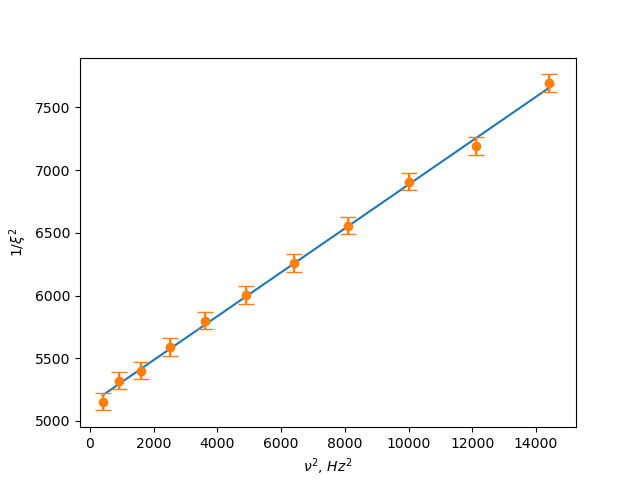
\includegraphics[width=0.6\pdfpagewidth]{graph1.png}
    \caption{График зависимости $1/\xi^2(\nu)$}
\end{figure}

\newpage

\subsection{Измерение проводимости через разность фаз в низкочастотном диапазоне}

Построим график $\tan{\psi}(\nu)$ по тем точкам точкам, для которых он хорошо аппроксимируется прямой

\begin{equation*}
    \tan{\psi} = k \cdot \nu 
\end{equation*}
\begin{equation*}
    k = \pi a h \sigma \mu_0
\end{equation*}

Отсюда получаем:

\begin{equation*}
    \sigma = (3.5 \pm 1.5) \cdot 10^7
\end{equation*}

\begin{figure}[h!]
    \centering
    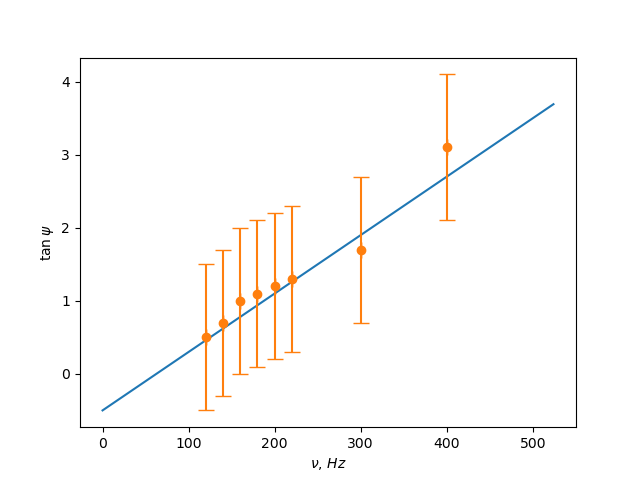
\includegraphics[width=0.6\pdfpagewidth]{graph3.png}
    \caption{График зависимости $\tan{\psi}(\nu)$}
\end{figure}

\subsection{Измерение проводимости через изменение индуктивности}

Измерить проводимость можно также через изменение индуктивности катушки внутри цилиндра

\begin{figure}[h!]
    \centering
    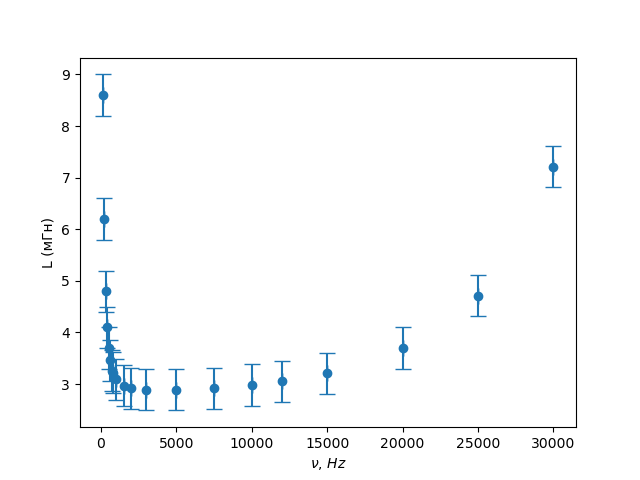
\includegraphics[width=0.6\pdfpagewidth]{graph4.png}
    \caption{График зависимости $L(\nu)$}
\end{figure}

\begin{figure}[h!]
    \centering
    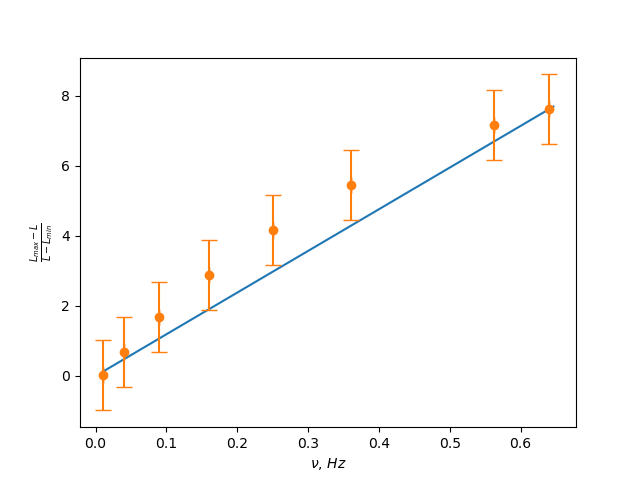
\includegraphics[width=0.6\pdfpagewidth]{graph2.png}
    \caption{График зависимости $\frac{L_{max} - L}{L - L_{min}}(\nu^2)$}
\end{figure}

\begin{equation*}
    L_{min} = 2.8 ~ \text{мГн}
\end{equation*}
\begin{equation*}
    L_{max} = 8.6 ~ \text{мГн}
\end{equation*}

	
То есть коэффициент наклона графика
\[k = (\pi ah\mu_0 \sigma)^2 \ \rightarrow \sigma = \frac{\sqrt{k}}{\pi ah \mu_0}\]

Подставляя полученные значения, получаем:

\begin{equation}
    \sigma = (4.3 \pm 0.2) \cdot 10^7  \ \frac{\text{См}}{\text{м}}
\end{equation}

\section{Вывод}

В ходе работы был исследован процесс проникновения переменного магнитного поля в медный полый цилиндр, и экспериментально определены значения удельной проводимости $\sigma$ меди тремя различными методами. Результаты измерений представлены в таблице:

\begin{table}[h!]
    \centering
    \begin{tabular}{|c|c|c|}
        \hline
        \textbf{Метод определения} & \textbf{Полученное значение $\sigma$, $10^7 \, \frac{\text{См}}{\text{м}}$} & \textbf{Погрешность, $\%$} \\ \hline
        По амплитудам & $4.5$ & $9$ \\ \hline
        По фазовому сдвигу & $3.5$ & $43$ \\ \hline
        По изменению индуктивности & $4.3$ & $5$ \\ \hline
    \end{tabular}
    \caption{Сравнение методов определения удельной проводимости $\sigma$}
\end{table}

Наиболее точным оказался метод измерения удельной проводимости через изменение индуктивности катушки внутри цилиндра, так как он дал наименьшую относительную погрешность ($\pm 5\%$). Метод измерения через амплитуды также показал приемлемый результат, близкий к табличному значению $\sigma \approx 5 \cdot 10^7 \, \frac{\text{См}}{\text{м}}$, с относительной погрешностью $9\%$. 

Наибольшая погрешность наблюдается при определении $\sigma$ через разность фаз ($\pm 43\%$), что можно объяснить крайне неточным методом измерения фазового сдвига.

Таким образом, полученные результаты совпали по порядку с табличным значением $\sigma$.


\end{document}
